\section{Estimating the time needed for a task}

\newcommand{\pois}{\ensuremath{\mathop{pois}}}
\newcommand{\tree}{\ensuremath{\mathop{tree}}}
\newcommand{\base}{\ensuremath{\mathop{base}}}
\newcommand{\child}{\ensuremath{\mathop{child}}}
\newcommand{\children}{\ensuremath{\mathop{children}}}
\newcommand{\GammaDist}{\ensuremath{\mathop{Gamma}}}
\newcommand{\var}{\ensuremath{\mathop{var}}}
\newcommand{\mean}{\ensuremath{\mathop{mean}}}


Lets model the growth of a tree like this: we begin with the trunk. From the trunk, branches may grow. How many branches is decided by a Poisson-distribution, whose expected number of branches is dependent on the height from the ground. 

\begin{lstlisting}[language=python]
from scipy.stats import poisson
from collections import namedtuple


Node = namedtuple('Node', 'parent, children')


def lamPerHeight(height):
    return 4 - height * 4 // 7


def randomTree(height=0):
    tree = Node(parent=None, children=[])
    lam = lamPerHeight(height)
    nrChildren = poisson.rvs(lam, size=1)
    for i in range(nrChildren):
        child = randomTree(height + 1)
        tree.children.append(child)
    return tree

print randomTree()
\end{lstlisting}

Using a Poisson-distribution, the probability of there being $k$ branches on height $h$ would be
$$ \pois_h(k) = \frac{ e^{-\lambda_h} \lambda_h^k }{ k! }$$

From the probability of a single branch we can now model the probabilty of a \tree. Consider the following \tree: 

\Tree[.n_1 [.n_2 n_3 ] n'_2 ] 

For this \tree the probability is $P(\tree) = \pois_1(2) \pois_2(1) \pois_3(0) \pois_2(0) $, or more generally:

$$ P(\tree) = \pois_1(|\children|) \prod_{\children} P(childtree)$$

\begin{lstlisting}[language=python]
def prob(tree, height=0):
    p = 1
    nrChildren = len(tree.children)
    lam = lamPerHeight(height)
    p *= poisson.pmf(nrChildren, lam)
    for child in tree.children:
        p *= prob(child, height + 1)
    return p


t = randomTree()
pt = prob(t)
\end{lstlisting}

Now what about this tree: 

\Tree[.n_1 [.n_2 [.n_3 ? ] ? ] [.n'_2 ? ] ? ] 

This is an unfinished tree. It's probability is $P(\{\tree | \tree_0 \subseteq \tree\}) = \pois_1(\geq2) \pois_2(\geq1) \pois_3(\geq0) \pois_2(\geq0) = \pois_1(\geq2) \pois_2(\geq1)$, or more generally: 

$$  P(\{\tree | \tree_0 \subseteq \tree\}) = \pois_1(\geq |\children|) \prod_{\children} P(\{ childtree | childtree_0 \subseteq childtree \}) $$

\begin{lstlisting}[language=python]
def probUnfinished(tree, height=0):
    p = 1
    nrChildren = len(tree.children)
    lam = lamPerHeight(height)
    p *= (1 - poisson.cdf(nrChildren, lam))
    for child in tree.children:
        p *= probUnfinished(child, height + 1)
    return p
\end{lstlisting}

\begin{figure}
  \caption{Using this model, we can spawn random trees}
  \centering
    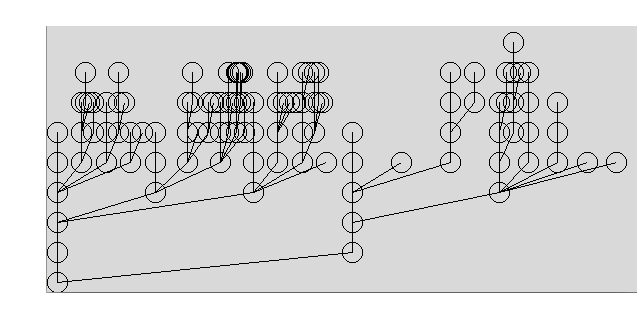
\includegraphics[width=0.5\textwidth]{images/randomtree.png}
\end{figure}

\paragraph{Time as random variable} 

Let time $T$ be a random variable of a tree $\tree$ defined as: 

$$ T_b(\tree) = T_n(\base) + \sum T_b(\child) $$

The expexted time for a not yet grown tree would then be:

$$ E[T_b] = \sum_{\tree \in \samplespace} T_b(\tree) P(\tree) $$

And the expected time given that we already have the fist few nodes of a tree:

$$ E[T_b]_{| \tree_0}  = \sum_{\tree \in \samplespace} T_b(\tree) P( \tree | \tree_0 )$$

This sum is pretty hard to compute, since \samplespace is an infinite set. But there is a way around this problem. Consider this tree: 

\Tree [.n_1 [.n_2 n_3 ] n'_2 ]

What is the expected number $k$ of nodes on level 2, given that there are already two offspring? 

$$ E[k] | k \geq 2 = \sum_{k=0}^\infty k P(k|2) =  \sum_{k=2}^\infty k \frac{ \pois_{\lambda_2}(k) }{ \pois_{\lambda_2}(\geq 2) }$$

$$ = \frac{1}{\pois_{\lambda_2}(\geq 2)} [ \sum_{k=0}^\infty k \pois_{\lambda_2}(k)  - \sum_{k=0}^1 k \pois_{\lambda_2}(k) ] $$

$$ = \frac{1}{\pois_{\lambda_2}(\geq 2)} [ E[k] - \sum_{k=0}^1 k \pois_{\lambda_2}(k) ]$$

$$ = \frac{\lambda - \sum_{k=0}^{k=1} k \pois_{\lambda_2}(k)}{1 - \sum_{k=0}^{k=1} \pois_{\lambda_2}(k)}$$

$$ = \frac{ \lambda - e^{-\lambda} \sum_{k=0}^{k=1} k \lambda^k / k! }{ 1 - e^{-\lambda} \sum_{k=0}^{k=1} \lambda^k / k! } $$


We can check our predictions numerically: 

\begin{lstlisting}[language=python]
from math import factorial, exp, floor


def pois(lmbd, k):
    return exp(-lmbd) * lmbd**k / factorial(k)


def poisCuml(lmbd, k):
    p = 0
    for j in range(k+1):
        p += pois(lmbd, j)
    return p


def poisCond(lmbd, k, k0):
    pb = 1 - poisCuml(lmbd, k0 - 1)
    if k < k0:
        pa = 0
    else:
        pa = pois(lmbd, k)
    return pa / pb


def expPois(lmbd):
    s = 0
    for i in range(int(50*lmbd)):
        s += i * pois(lmbd, i)
    return s


def expPoisCond(lmbd, k0):
    e = 0
    for i in range(k0, int(50*lmbd)):
        e += i * poisCond(lmbd, i, k0)
    return e


def expPoisCondAnal(lmbd, k0):
    sum1 = sum2 = 0
    for k in range(k0 + 1):
        sum1 += k * lmbd**k / float(factorial(k))
    for k in range(k0 + 1):
        sum2 += lmbd**k / float(factorial(k))
    sum1 *= exp(-lmbd)
    sum2 *= exp(-lmbd)
    a = float(lmbd - sum1)
    b = float(1 - sum2)
    return a / b

\end{lstlisting}


We will make use of this result shortly.

\begin{figure}
  \caption{When we already have 6 nodes, the probability of getting new nodes changes}
  \centering
    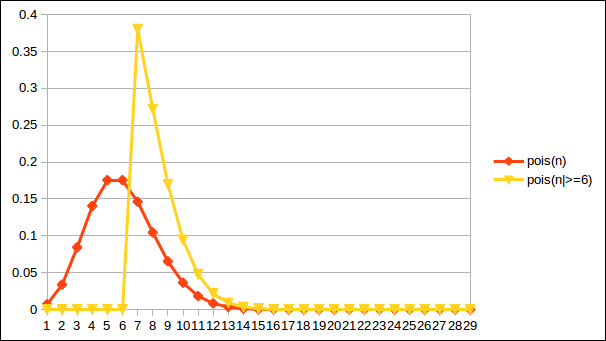
\includegraphics[width=0.5\textwidth]{images/conditional_poisson.png}
\end{figure}





We can use this to find an intuitive expression for $E[T_b(\tree)]$, which would be: 

$$ E[T_b(\tree)]_{| \tree_0} = E[T_n(\base) + \sum T_b(\child)]_{| \tree_0} $$

$$ = E[T_n(\base)]_{| \tree_0} + E[ \sum T_b(\child) ]_{| \tree_0} $$

The term $ E[ \sum T_b(\child) ]_{| \tree_0} $ is somewhat special: we cannot just equal it to $  \sum E[ T_b(\child) ]_{|\tree_0} $, because we don't yet know how many children the tree will have. But it is reasonable to assume that:

$$ E[ \sum T_b(\child) ]_{| \tree_0} = \sum_{children_0} E[T_b(\child)] + \sum_{E[|\children|]_{ \children_0} - \children_0} E[T_b(\child)] $$

With this, the previous equation becomes: 

$$ E[T_b(\tree)]_{| \tree_0} = E[T_n(\base)]_{| \tree_0} +  \sum_{\children_0} E[T_b(\child)] + \sum_{E[|\children|]_{ \children_0} - \children_0} E[T_b(\child)] $$

Now there are a bunch of terms in this equation that we can approximate statistically: 

\begin{itemize}

    \item $ E[|\children|]_{| \children_0} = \frac{ \lambda - e^{-\lambda} \sum_{k=0}^{k=\children_0 - 1} k \lambda^k / k! }{ 1 - e^{-\lambda} \sum_{k=0}^{k=\children_0 - 1} \lambda^k / k! }  $. Here we can approximate $\lambda$ by the average number of children on this level.
    
    \item $ E[T_n(\base)]_{| \tree_0} $ can be approximated by the average net-time on this level
    
    \item $ E[T_b(\child)] $ knows two cases: 
    
        \begin{itemize}
            
            \item if we're dealing with a real child, the value is approximated with the same formula applied recursively 
            
            \item if we're dealing with a not-yet-spawned child, we have: $ E[T_b] = E[T_n(1)] + E[\#c1] E[T_n(2)] + E[\#c1]E[\#c2]E[T_n(3)] + E[\#c1]E[\#c2]E[\#n3]E[T_n(4)] + ... $
        \end{itemize}

\end{itemize}


\paragraph{Time as random variable: revisited}

We can enhance our model quite a bit by recognizing that $T_b(\base)$ is not a constant, but a random variable in its own right. 

Then this random variable would still be defined as: 

$$ T_b(\tree) = T_n(\base) + \sum T_b(\child) $$

But $T_n(\base)$ itself would be random as well. 

Under these assumptions, we get: 

$$ P(t | t_0) = \{ \begin{array}{lr}
        \frac{P(t)}{1 - P(t<t_0)}       & \text{for } t \geq t_0 \\
        0                               & \text{for }  t < t_0
        \end{array}  $$

$$ E[T_n(\base)]_{|t_0} = \int_0^\infty t P(t|t\geq t_0) \diff{t} $$

$$ = \frac{1}{1 - P(t|t<t_0)} \int_{t_0}^\infty t P(t) \diff{t} $$

$$ = \frac{1}{1 - P(t|t<t_0)} [ E[t] - \int_0^{t_0} t P(t) \diff{t} ] $$

Assuming that $P(t) = \GammaDist_{\alpha,\beta}(t) = \frac{\beta^\alpha e^{-\beta} t^{\alpha-1} }{\Gamma(\alpha) } $, we obtain: 

$$ \int_0^{t_0} t P(t) \diff{t} = \frac{\beta^\alpha e^{-\beta} }{\Gamma(\alpha) } \int_0^{t_0} t^{\alpha - 1} t \diff{t} $$

$$ =  \frac{\beta^\alpha e^{-\beta} t_0^{\alpha-1} }{\Gamma(\alpha) }  \frac{t_0^2}{\alpha + 1} = \GammaDist_{\alpha, \beta}(t_0) \frac{t_0^2}{\alpha + 1} $$


Here, the parameters $\alpha$ and $\beta$ can be estimated by: 

$$ \alpha \approx \frac{\mean(t) \mean(t)}{\var(t)} $$
$$ \beta \approx \frac{\mean(t)}{\var(t)} $$


We can once again verify this model numerically: 

\begin{lstlisting}[language=python]
import scipy as sp
from scipy.stats import gamma
import matplotlib.pyplot as plt


def rateToScale(beta):
    return 1/beta

def scaleToRate(theta):
    return 1/theta

def probGamma(t, alpha, beta):
    theta = rateToScale(beta)
    return gamma.pdf(t, a=alpha, scale=theta)

def probGammaCond(t, t0, alpha, beta):
    theta = rateToScale(beta)
    gam = gamma(a=alpha, scale=theta)
    tpart1 = t[sp.where(t<t0)]
    outpart1 = sp.zeros(sp.shape(tpart1))
    tpart2 = t[sp.where(t>=t0)]
    pt = gam.pdf(tpart2)
    Pt0 = gam.cdf(t0)
    outpart2 = pt / (1 - Pt0 )
    return sp.concatenate([outpart1, outpart2])

def expGammaCond(t0, alpha, beta):
    theta = rateToScale(beta)
    gam = gamma(a=alpha, scale=theta)
    expv = gam.mean()
    gt0 = gam.pdf(t0)
    gfac = t0 * t0 / (alpha + 1)
    gCumt0 = gam.cdf(t0)
    return ( expv - gt0 * gfac ) / ( 1 - gCumt0 )

mean = 3.0
var = 2.0
alpha = mean * mean / var
beta = mean / var
t0  = 4
t = sp.arange(0, 10, 0.1)
pn = probGamma(t, alpha, beta)
pc = probGammaCond(t, t0, alpha, beta)


plt.plot(t, pn)
plt.plot(t, pc)
plt.show()
\end{lstlisting}


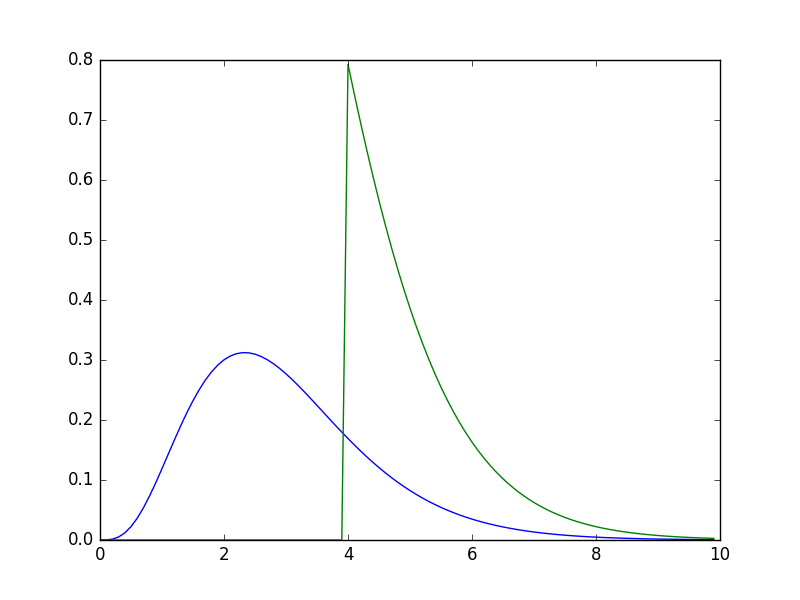
\includegraphics[width=0.5\textwidth]{images/beta_conditional.png}


This model justifies another look at our samplespace. Note that ....
